\documentclass[twoside]{book}

% Packages required by doxygen
\usepackage{calc}
\usepackage{doxygen}
\usepackage{graphicx}
\usepackage[utf8]{inputenc}
\usepackage{makeidx}
\usepackage{multicol}
\usepackage{multirow}
\usepackage{textcomp}
\usepackage[table]{xcolor}

% Font selection
\usepackage[T1]{fontenc}
\usepackage{mathptmx}
\usepackage[scaled=.90]{helvet}
\usepackage{courier}
\usepackage{amssymb}
\usepackage{sectsty}
\renewcommand{\familydefault}{\sfdefault}
\allsectionsfont{%
  \fontseries{bc}\selectfont%
  \color{darkgray}%
}
\renewcommand{\DoxyLabelFont}{%
  \fontseries{bc}\selectfont%
  \color{darkgray}%
}

% Page & text layout
\usepackage{geometry}
\geometry{%
  a4paper,%
  top=2.5cm,%
  bottom=2.5cm,%
  left=2.5cm,%
  right=2.5cm%
}
\tolerance=750
\hfuzz=15pt
\hbadness=750
\setlength{\emergencystretch}{15pt}
\setlength{\parindent}{0cm}
\setlength{\parskip}{0.2cm}
\makeatletter
\renewcommand{\paragraph}{%
  \@startsection{paragraph}{4}{0ex}{-1.0ex}{1.0ex}{%
    \normalfont\normalsize\bfseries\SS@parafont%
  }%
}
\renewcommand{\subparagraph}{%
  \@startsection{subparagraph}{5}{0ex}{-1.0ex}{1.0ex}{%
    \normalfont\normalsize\bfseries\SS@subparafont%
  }%
}
\makeatother

% Headers & footers
\usepackage{fancyhdr}
\pagestyle{fancyplain}
\fancyhead[LE]{\fancyplain{}{\bfseries\thepage}}
\fancyhead[CE]{\fancyplain{}{}}
\fancyhead[RE]{\fancyplain{}{\bfseries\leftmark}}
\fancyhead[LO]{\fancyplain{}{\bfseries\rightmark}}
\fancyhead[CO]{\fancyplain{}{}}
\fancyhead[RO]{\fancyplain{}{\bfseries\thepage}}
\fancyfoot[LE]{\fancyplain{}{}}
\fancyfoot[CE]{\fancyplain{}{}}
\fancyfoot[RE]{\fancyplain{}{\bfseries\scriptsize Generated on Thu Mar 16 2017 13\-:16\-:09 for I\-N101 project on Conway's Game of Life by Doxygen }}
\fancyfoot[LO]{\fancyplain{}{\bfseries\scriptsize Generated on Thu Mar 16 2017 13\-:16\-:09 for I\-N101 project on Conway's Game of Life by Doxygen }}
\fancyfoot[CO]{\fancyplain{}{}}
\fancyfoot[RO]{\fancyplain{}{}}
\renewcommand{\footrulewidth}{0.4pt}
\renewcommand{\chaptermark}[1]{%
  \markboth{#1}{}%
}
\renewcommand{\sectionmark}[1]{%
  \markright{\thesection\ #1}%
}

% Indices & bibliography
\usepackage{natbib}
\usepackage[titles]{tocloft}
\setcounter{tocdepth}{3}
\setcounter{secnumdepth}{5}
\makeindex

% Hyperlinks (required, but should be loaded last)
\usepackage{ifpdf}
\ifpdf
  \usepackage[pdftex,pagebackref=true]{hyperref}
\else
  \usepackage[ps2pdf,pagebackref=true]{hyperref}
\fi
\hypersetup{%
  colorlinks=true,%
  linkcolor=blue,%
  citecolor=blue,%
  unicode%
}

% Custom commands
\newcommand{\clearemptydoublepage}{%
  \newpage{\pagestyle{empty}\cleardoublepage}%
}


%===== C O N T E N T S =====

\begin{document}

% Titlepage & ToC
\hypersetup{pageanchor=false}
\pagenumbering{roman}
\begin{titlepage}
\vspace*{7cm}
\begin{center}%
{\Large I\-N101 project on Conway's Game of Life }\\
\vspace*{1cm}
{\large Generated by Doxygen 1.8.5}\\
\vspace*{0.5cm}
{\small Thu Mar 16 2017 13:16:09}\\
\end{center}
\end{titlepage}
\clearemptydoublepage
\tableofcontents
\clearemptydoublepage
\pagenumbering{arabic}
\hypersetup{pageanchor=true}

%--- Begin generated contents ---
\chapter{Class Index}
\section{Class List}
Here are the classes, structs, unions and interfaces with brief descriptions\-:\begin{DoxyCompactList}
\item\contentsline{section}{\hyperlink{structcell}{cell} }{\pageref{structcell}}{}
\item\contentsline{section}{\hyperlink{structcoordinate}{coordinate} }{\pageref{structcoordinate}}{}
\item\contentsline{section}{\hyperlink{structproblem}{problem} }{\pageref{structproblem}}{}
\end{DoxyCompactList}

\chapter{File Index}
\section{File List}
Here is a list of all documented files with brief descriptions\-:\begin{DoxyCompactList}
\item\contentsline{section}{include/\hyperlink{cell_8h}{cell.\-h} \\*Definition of the problem, the population and cells }{\pageref{cell_8h}}{}
\item\contentsline{section}{include/\hyperlink{generate-image_8h}{generate-\/image.\-h} \\*Enable to generate an image }{\pageref{generate-image_8h}}{}
\item\contentsline{section}{include/\hyperlink{load_8h}{load.\-h} \\*Enable to load an image }{\pageref{load_8h}}{}
\end{DoxyCompactList}

\chapter{Class Documentation}
\hypertarget{structcell}{\section{cell Struct Reference}
\label{structcell}\index{cell@{cell}}
}


Collaboration diagram for cell\-:\nopagebreak
\begin{figure}[H]
\begin{center}
\leavevmode
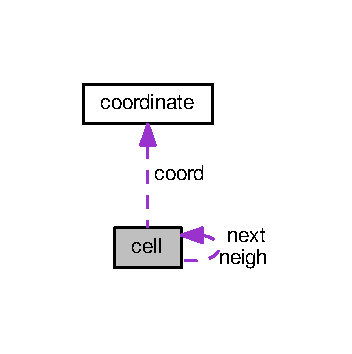
\includegraphics[width=169pt]{structcell__coll__graph}
\end{center}
\end{figure}
\subsection*{Public Attributes}
\begin{DoxyCompactItemize}
\item 
\hypertarget{structcell_ab170fb0ebb0c01838beb95b2b2505f58}{\hyperlink{cell_8h_a015eb90e0de9f16e87bd149d4b9ce959}{status} {\bfseries stat}}\label{structcell_ab170fb0ebb0c01838beb95b2b2505f58}

\item 
\hypertarget{structcell_ad6089b3f9838a549e0664db6ad4d77cb}{\hyperlink{structcoordinate}{coordinate} {\bfseries coord}}\label{structcell_ad6089b3f9838a549e0664db6ad4d77cb}

\item 
\hypertarget{structcell_ad74bc65d9825fe95f7b0f31eae74ef9b}{\hyperlink{structcell}{cell} $\ast$ {\bfseries neigh} \mbox{[}8\mbox{]}}\label{structcell_ad74bc65d9825fe95f7b0f31eae74ef9b}

\item 
\hypertarget{structcell_a99a5ca970a81fe153b1007165617e066}{\hyperlink{structcell}{cell} $\ast$ {\bfseries next}}\label{structcell_a99a5ca970a81fe153b1007165617e066}

\end{DoxyCompactItemize}


The documentation for this struct was generated from the following file\-:\begin{DoxyCompactItemize}
\item 
include/\hyperlink{cell_8h}{cell.\-h}\end{DoxyCompactItemize}

\hypertarget{structcoordinate}{\section{coordinate Struct Reference}
\label{structcoordinate}\index{coordinate@{coordinate}}
}
\subsection*{Public Attributes}
\begin{DoxyCompactItemize}
\item 
\hypertarget{structcoordinate_a8480dda1b2992713d4b0750bbdf1ee4e}{int {\bfseries x}}\label{structcoordinate_a8480dda1b2992713d4b0750bbdf1ee4e}

\item 
\hypertarget{structcoordinate_a1f90088affc8f61daa374403f148eeb7}{int {\bfseries y}}\label{structcoordinate_a1f90088affc8f61daa374403f148eeb7}

\end{DoxyCompactItemize}


The documentation for this struct was generated from the following file\-:\begin{DoxyCompactItemize}
\item 
include/\hyperlink{cell_8h}{cell.\-h}\end{DoxyCompactItemize}

\hypertarget{structproblem}{\section{problem Struct Reference}
\label{structproblem}\index{problem@{problem}}
}


Collaboration diagram for problem\-:\nopagebreak
\begin{figure}[H]
\begin{center}
\leavevmode
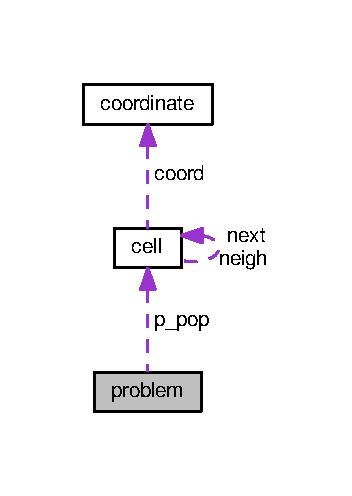
\includegraphics[width=169pt]{structproblem__coll__graph}
\end{center}
\end{figure}
\subsection*{Public Attributes}
\begin{DoxyCompactItemize}
\item 
\hypertarget{structproblem_af1181ee7cfe4becf4d9474d254852c88}{int {\bfseries grid\-\_\-size} \mbox{[}2\mbox{]}}\label{structproblem_af1181ee7cfe4becf4d9474d254852c88}

\item 
\hypertarget{structproblem_a0f678c7f2aff7a1104141a3f5fe4f216}{int {\bfseries number\-\_\-of\-\_\-steps}}\label{structproblem_a0f678c7f2aff7a1104141a3f5fe4f216}

\item 
\hypertarget{structproblem_a840047e720ee20d193f686894c2de764}{\hyperlink{cell_8h_a9b7e2581d2e2f2fc3d141d599d3b11e3}{population} $\ast$ {\bfseries p\-\_\-pop}}\label{structproblem_a840047e720ee20d193f686894c2de764}

\end{DoxyCompactItemize}


The documentation for this struct was generated from the following file\-:\begin{DoxyCompactItemize}
\item 
include/\hyperlink{cell_8h}{cell.\-h}\end{DoxyCompactItemize}

\chapter{File Documentation}
\hypertarget{cell_8h}{\section{include/cell.h File Reference}
\label{cell_8h}\index{include/cell.\-h@{include/cell.\-h}}
}


Definition of the problem, the population and cells.  


{\ttfamily \#include $<$stdio.\-h$>$}\\*
{\ttfamily \#include $<$stdlib.\-h$>$}\\*
{\ttfamily \#include $<$stdbool.\-h$>$}\\*
{\ttfamily \#include $<$string.\-h$>$}\\*
{\ttfamily \#include $<$error.\-h$>$}\\*
Include dependency graph for cell.\-h\-:\nopagebreak
\begin{figure}[H]
\begin{center}
\leavevmode
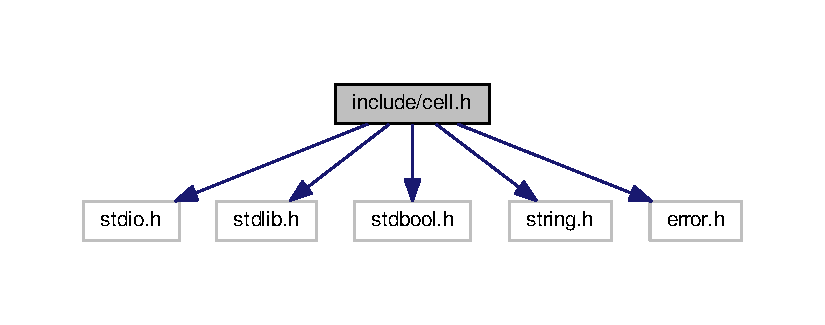
\includegraphics[width=350pt]{cell_8h__incl}
\end{center}
\end{figure}
This graph shows which files directly or indirectly include this file\-:\nopagebreak
\begin{figure}[H]
\begin{center}
\leavevmode
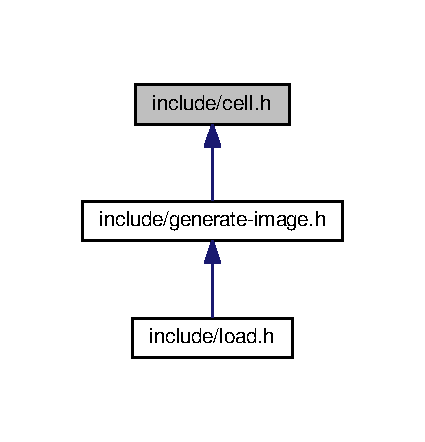
\includegraphics[width=204pt]{cell_8h__dep__incl}
\end{center}
\end{figure}
\subsection*{Classes}
\begin{DoxyCompactItemize}
\item 
struct \hyperlink{structcoordinate}{coordinate}
\item 
struct \hyperlink{structcell}{cell}
\item 
struct \hyperlink{structproblem}{problem}
\end{DoxyCompactItemize}
\subsection*{Typedefs}
\begin{DoxyCompactItemize}
\item 
\hypertarget{cell_8h_ac0e5b7b5b4d698de3f31f6644ca0a94e}{typedef struct \hyperlink{structcoordinate}{coordinate} \hyperlink{cell_8h_ac0e5b7b5b4d698de3f31f6644ca0a94e}{coordinate}}\label{cell_8h_ac0e5b7b5b4d698de3f31f6644ca0a94e}

\begin{DoxyCompactList}\small\item\em A structure representing the coordinate of a point in a plane. \end{DoxyCompactList}\item 
\hypertarget{cell_8h_aec1b5e3c3df16427325defaffcb3cb2e}{typedef struct \hyperlink{structcell}{cell} \hyperlink{cell_8h_aec1b5e3c3df16427325defaffcb3cb2e}{cell}}\label{cell_8h_aec1b5e3c3df16427325defaffcb3cb2e}

\begin{DoxyCompactList}\small\item\em A structure representing a cell. \end{DoxyCompactList}\item 
\hypertarget{cell_8h_a9b7e2581d2e2f2fc3d141d599d3b11e3}{typedef struct \hyperlink{structcell}{cell} $\ast$ \hyperlink{cell_8h_a9b7e2581d2e2f2fc3d141d599d3b11e3}{population}}\label{cell_8h_a9b7e2581d2e2f2fc3d141d599d3b11e3}

\begin{DoxyCompactList}\small\item\em A structure representing a population. \end{DoxyCompactList}\item 
\hypertarget{cell_8h_a8f761a52800d0c65186c16662a1197a7}{typedef struct \hyperlink{structproblem}{problem} \hyperlink{cell_8h_a8f761a52800d0c65186c16662a1197a7}{problem}}\label{cell_8h_a8f761a52800d0c65186c16662a1197a7}

\begin{DoxyCompactList}\small\item\em A structure representing a problem. \end{DoxyCompactList}\end{DoxyCompactItemize}
\subsection*{Enumerations}
\begin{DoxyCompactItemize}
\item 
enum \hyperlink{cell_8h_a015eb90e0de9f16e87bd149d4b9ce959}{status} \{ {\bfseries A\-L\-I\-V\-E}, 
{\bfseries N\-E\-W\-B\-O\-R\-N}, 
{\bfseries D\-Y\-I\-N\-G}
 \}
\begin{DoxyCompactList}\small\item\em An enumeration which contains the different possible status of a cell. \end{DoxyCompactList}\end{DoxyCompactItemize}
\subsection*{Functions}
\begin{DoxyCompactItemize}
\item 
int \hyperlink{cell_8h_a9b2a7ea0c749e21682f08bf8099b73b7}{iindex} (int index)
\begin{DoxyCompactList}\small\item\em Return the reciprocal index of two neighbouring cells. \end{DoxyCompactList}\item 
\hyperlink{cell_8h_a9b7e2581d2e2f2fc3d141d599d3b11e3}{population} \hyperlink{cell_8h_ad85e7100d3e86c427851f8b27e303aa5}{nil} (void)
\begin{DoxyCompactList}\small\item\em Return an empty population. \end{DoxyCompactList}\item 
void \hyperlink{cell_8h_a779fb98cabdc5e91d776de8c195d8169}{add\-\_\-cell} (\hyperlink{structproblem}{problem} $\ast$p\-\_\-prob, \hyperlink{structcoordinate}{coordinate} coord, \hyperlink{cell_8h_a015eb90e0de9f16e87bd149d4b9ce959}{status} stat)
\begin{DoxyCompactList}\small\item\em Add a cell to a population. \end{DoxyCompactList}\item 
void \hyperlink{cell_8h_af601d4688b7489ae7753bd45f61e0b24}{remove\-\_\-cell} (\hyperlink{structproblem}{problem} $\ast$p\-\_\-prob, \hyperlink{structcoordinate}{coordinate} coord)
\begin{DoxyCompactList}\small\item\em Remove a cell from a population. \end{DoxyCompactList}\item 
bool \hyperlink{cell_8h_aaa4216c60537c08296db2da595b47b2d}{is\-\_\-neighbor} (\hyperlink{structproblem}{problem} $\ast$p\-\_\-prob, \hyperlink{structcoordinate}{coordinate} coord1, \hyperlink{structcoordinate}{coordinate} coord2)
\begin{DoxyCompactList}\small\item\em Enables to know if two cells are neighbor considering their coordinates. \end{DoxyCompactList}\item 
\hyperlink{structcoordinate}{coordinate} \hyperlink{cell_8h_a736e96dec4f5a5abf45dd11b5789c202}{neighbor} (\hyperlink{structproblem}{problem} $\ast$p\-\_\-prob, \hyperlink{structcell}{cell} $\ast$p\-\_\-cell, int index)
\begin{DoxyCompactList}\small\item\em Enables to know the coordinates of the neighbor of index i of a cell considering the edges of the game. \end{DoxyCompactList}\item 
\hyperlink{structcell}{cell} $\ast$ \hyperlink{cell_8h_aa8682a66e00f6057274d888f4f88731b}{find\-\_\-cell} (\hyperlink{structproblem}{problem} $\ast$p\-\_\-prob, \hyperlink{structcoordinate}{coordinate} coord)
\begin{DoxyCompactList}\small\item\em Find a cell in a population. \end{DoxyCompactList}\item 
void \hyperlink{cell_8h_a0e6598e1dcfe64bd21d1fd4c3873eba2}{next\-\_\-generation} (\hyperlink{structproblem}{problem} $\ast$p\-\_\-prob)
\begin{DoxyCompactList}\small\item\em Update the population to the population's next generation. \end{DoxyCompactList}\item 
void \hyperlink{cell_8h_a3c16dc610ff30371be993d99139d90e5}{deallocate\-\_\-population} (\hyperlink{structproblem}{problem} $\ast$p\-\_\-prob)
\begin{DoxyCompactList}\small\item\em Free the memomy allocated to a population. \end{DoxyCompactList}\item 
void \hyperlink{cell_8h_a3bfbe7ddc8923cf3e35230a7fec1af57}{deallocate\-\_\-problem} (\hyperlink{structproblem}{problem} $\ast$p\-\_\-prob)
\begin{DoxyCompactList}\small\item\em Free the memomy allocated to a problem. \end{DoxyCompactList}\item 
void \hyperlink{cell_8h_a56e6216bdd71d675126d7a972257ba78}{print\-\_\-pop} (\hyperlink{structproblem}{problem} $\ast$p\-\_\-prob)
\begin{DoxyCompactList}\small\item\em print the whole population \end{DoxyCompactList}\end{DoxyCompactItemize}


\subsection{Detailed Description}
Definition of the problem, the population and cells. \begin{DoxyAuthor}{Author}
Maxence Faldor
\end{DoxyAuthor}
Defines different structures\-:
\begin{DoxyItemize}
\item a structure coordinate
\item a structure cell
\item a structure population which is a linked list of cells
\item a structure problem containing all the parameters of the conway problem
\end{DoxyItemize}

Contains useful functions\-:
\begin{DoxyItemize}
\item a function to return the reciprocal index of two neighbouring cells
\item a function to create a empty population
\item a function to add a cell to a population
\item a function to remove a cell from a population
\item a function to know if two cells are neighbor considering their coordinates
\item a function to return the coordinate of the neighbor of index i of a cell
\item a function to get the adress of a cell in the population
\item a function to get the population's next generation
\item a function to deallocate a population
\item a function to deallocate a problem
\item a function to print a population 
\end{DoxyItemize}

\subsection{Function Documentation}
\hypertarget{cell_8h_a779fb98cabdc5e91d776de8c195d8169}{\index{cell.\-h@{cell.\-h}!add\-\_\-cell@{add\-\_\-cell}}
\index{add\-\_\-cell@{add\-\_\-cell}!cell.h@{cell.\-h}}
\subsubsection[{add\-\_\-cell}]{\setlength{\rightskip}{0pt plus 5cm}void add\-\_\-cell (
\begin{DoxyParamCaption}
\item[{{\bf problem} $\ast$}]{p\-\_\-prob, }
\item[{{\bf coordinate}}]{coord, }
\item[{{\bf status}}]{stat}
\end{DoxyParamCaption}
)}}\label{cell_8h_a779fb98cabdc5e91d776de8c195d8169}


Add a cell to a population. 


\begin{DoxyParams}{Parameters}
{\em p\-\_\-prob} & a pointer to the problem. \\
\hline
{\em coord} & coordinates of the new cell. \\
\hline
{\em stat} & status of the new cell.\\
\hline
\end{DoxyParams}
\begin{DoxyPostcond}{Postcondition}
A new cell is added to a population with its parameters. Neighbors of each cell are updated. 
\end{DoxyPostcond}
\hypertarget{cell_8h_a3c16dc610ff30371be993d99139d90e5}{\index{cell.\-h@{cell.\-h}!deallocate\-\_\-population@{deallocate\-\_\-population}}
\index{deallocate\-\_\-population@{deallocate\-\_\-population}!cell.h@{cell.\-h}}
\subsubsection[{deallocate\-\_\-population}]{\setlength{\rightskip}{0pt plus 5cm}void deallocate\-\_\-population (
\begin{DoxyParamCaption}
\item[{{\bf problem} $\ast$}]{p\-\_\-prob}
\end{DoxyParamCaption}
)}}\label{cell_8h_a3c16dc610ff30371be993d99139d90e5}


Free the memomy allocated to a population. 


\begin{DoxyParams}{Parameters}
{\em p\-\_\-prob} & a pointer to the problem.\\
\hline
\end{DoxyParams}
\begin{DoxyPostcond}{Postcondition}
Each cell composing the population are freed. The population is deallocated. 
\end{DoxyPostcond}
\hypertarget{cell_8h_a3bfbe7ddc8923cf3e35230a7fec1af57}{\index{cell.\-h@{cell.\-h}!deallocate\-\_\-problem@{deallocate\-\_\-problem}}
\index{deallocate\-\_\-problem@{deallocate\-\_\-problem}!cell.h@{cell.\-h}}
\subsubsection[{deallocate\-\_\-problem}]{\setlength{\rightskip}{0pt plus 5cm}void deallocate\-\_\-problem (
\begin{DoxyParamCaption}
\item[{{\bf problem} $\ast$}]{p\-\_\-prob}
\end{DoxyParamCaption}
)}}\label{cell_8h_a3bfbe7ddc8923cf3e35230a7fec1af57}


Free the memomy allocated to a problem. 


\begin{DoxyParams}{Parameters}
{\em p\-\_\-prob} & a pointer to the problem.\\
\hline
\end{DoxyParams}
\begin{DoxyPostcond}{Postcondition}
All the memory allocated is freed. 
\end{DoxyPostcond}
\hypertarget{cell_8h_aa8682a66e00f6057274d888f4f88731b}{\index{cell.\-h@{cell.\-h}!find\-\_\-cell@{find\-\_\-cell}}
\index{find\-\_\-cell@{find\-\_\-cell}!cell.h@{cell.\-h}}
\subsubsection[{find\-\_\-cell}]{\setlength{\rightskip}{0pt plus 5cm}{\bf cell}$\ast$ find\-\_\-cell (
\begin{DoxyParamCaption}
\item[{{\bf problem} $\ast$}]{p\-\_\-prob, }
\item[{{\bf coordinate}}]{coord}
\end{DoxyParamCaption}
)}}\label{cell_8h_aa8682a66e00f6057274d888f4f88731b}


Find a cell in a population. 


\begin{DoxyParams}{Parameters}
{\em p\-\_\-prob} & a pointer to the problem. \\
\hline
{\em coord} & coordinates of the first cell.\\
\hline
\end{DoxyParams}
\begin{DoxyReturn}{Returns}
A pointer to the cell of coordinates coord if it belongs to the population. N\-U\-L\-L otherwise. 
\end{DoxyReturn}
\hypertarget{cell_8h_a9b2a7ea0c749e21682f08bf8099b73b7}{\index{cell.\-h@{cell.\-h}!iindex@{iindex}}
\index{iindex@{iindex}!cell.h@{cell.\-h}}
\subsubsection[{iindex}]{\setlength{\rightskip}{0pt plus 5cm}int iindex (
\begin{DoxyParamCaption}
\item[{int}]{index}
\end{DoxyParamCaption}
)}}\label{cell_8h_a9b2a7ea0c749e21682f08bf8099b73b7}


Return the reciprocal index of two neighbouring cells. 


\begin{DoxyParams}{Parameters}
{\em index} & The index of the neighbouring cell.\\
\hline
\end{DoxyParams}
\begin{DoxyReturn}{Returns}
The reciprocal index of two neighbouring cells. 
\end{DoxyReturn}
\hypertarget{cell_8h_aaa4216c60537c08296db2da595b47b2d}{\index{cell.\-h@{cell.\-h}!is\-\_\-neighbor@{is\-\_\-neighbor}}
\index{is\-\_\-neighbor@{is\-\_\-neighbor}!cell.h@{cell.\-h}}
\subsubsection[{is\-\_\-neighbor}]{\setlength{\rightskip}{0pt plus 5cm}bool is\-\_\-neighbor (
\begin{DoxyParamCaption}
\item[{{\bf problem} $\ast$}]{p\-\_\-prob, }
\item[{{\bf coordinate}}]{coord1, }
\item[{{\bf coordinate}}]{coord2}
\end{DoxyParamCaption}
)}}\label{cell_8h_aaa4216c60537c08296db2da595b47b2d}


Enables to know if two cells are neighbor considering their coordinates. 


\begin{DoxyParams}{Parameters}
{\em p\-\_\-prob} & a pointer to the problem. \\
\hline
{\em coord1} & coordinates of the first cell. \\
\hline
{\em coord2} & coordinates of the second cell.\\
\hline
\end{DoxyParams}
\begin{DoxyReturn}{Returns}
True if the cells are neighbouring. False otherwise. 
\end{DoxyReturn}
\hypertarget{cell_8h_a736e96dec4f5a5abf45dd11b5789c202}{\index{cell.\-h@{cell.\-h}!neighbor@{neighbor}}
\index{neighbor@{neighbor}!cell.h@{cell.\-h}}
\subsubsection[{neighbor}]{\setlength{\rightskip}{0pt plus 5cm}{\bf coordinate} neighbor (
\begin{DoxyParamCaption}
\item[{{\bf problem} $\ast$}]{p\-\_\-prob, }
\item[{{\bf cell} $\ast$}]{p\-\_\-cell, }
\item[{int}]{index}
\end{DoxyParamCaption}
)}}\label{cell_8h_a736e96dec4f5a5abf45dd11b5789c202}


Enables to know the coordinates of the neighbor of index i of a cell considering the edges of the game. 


\begin{DoxyParams}{Parameters}
{\em p\-\_\-prob} & a pointer to the problem. \\
\hline
{\em my\-\_\-cell} & a cell representing the reference. \\
\hline
{\em index} & the index of the considered neighbor.\\
\hline
\end{DoxyParams}
\begin{DoxyReturn}{Returns}
True if they are neighbouring cells. False otherwise. 
\end{DoxyReturn}
\hypertarget{cell_8h_a0e6598e1dcfe64bd21d1fd4c3873eba2}{\index{cell.\-h@{cell.\-h}!next\-\_\-generation@{next\-\_\-generation}}
\index{next\-\_\-generation@{next\-\_\-generation}!cell.h@{cell.\-h}}
\subsubsection[{next\-\_\-generation}]{\setlength{\rightskip}{0pt plus 5cm}void next\-\_\-generation (
\begin{DoxyParamCaption}
\item[{{\bf problem} $\ast$}]{p\-\_\-prob}
\end{DoxyParamCaption}
)}}\label{cell_8h_a0e6598e1dcfe64bd21d1fd4c3873eba2}


Update the population to the population's next generation. 


\begin{DoxyParams}{Parameters}
{\em p\-\_\-prob} & a pointer to the problem.\\
\hline
\end{DoxyParams}
\begin{DoxyPostcond}{Postcondition}
The population is changed according to the rules of the Conway's Game of Life. 
\end{DoxyPostcond}
\hypertarget{cell_8h_ad85e7100d3e86c427851f8b27e303aa5}{\index{cell.\-h@{cell.\-h}!nil@{nil}}
\index{nil@{nil}!cell.h@{cell.\-h}}
\subsubsection[{nil}]{\setlength{\rightskip}{0pt plus 5cm}{\bf population} nil (
\begin{DoxyParamCaption}
\item[{void}]{}
\end{DoxyParamCaption}
)}}\label{cell_8h_ad85e7100d3e86c427851f8b27e303aa5}


Return an empty population. 

\begin{DoxyReturn}{Returns}
An empty population. 
\end{DoxyReturn}
\hypertarget{cell_8h_a56e6216bdd71d675126d7a972257ba78}{\index{cell.\-h@{cell.\-h}!print\-\_\-pop@{print\-\_\-pop}}
\index{print\-\_\-pop@{print\-\_\-pop}!cell.h@{cell.\-h}}
\subsubsection[{print\-\_\-pop}]{\setlength{\rightskip}{0pt plus 5cm}void print\-\_\-pop (
\begin{DoxyParamCaption}
\item[{{\bf problem} $\ast$}]{p\-\_\-prob}
\end{DoxyParamCaption}
)}}\label{cell_8h_a56e6216bdd71d675126d7a972257ba78}


print the whole population 


\begin{DoxyParams}{Parameters}
{\em p\-\_\-prob} & a pointer to the problem.\\
\hline
\end{DoxyParams}
\begin{DoxyPostcond}{Postcondition}
Each cell composing the populaton is printed in the terminal. 
\end{DoxyPostcond}
\hypertarget{cell_8h_af601d4688b7489ae7753bd45f61e0b24}{\index{cell.\-h@{cell.\-h}!remove\-\_\-cell@{remove\-\_\-cell}}
\index{remove\-\_\-cell@{remove\-\_\-cell}!cell.h@{cell.\-h}}
\subsubsection[{remove\-\_\-cell}]{\setlength{\rightskip}{0pt plus 5cm}void remove\-\_\-cell (
\begin{DoxyParamCaption}
\item[{{\bf problem} $\ast$}]{p\-\_\-prob, }
\item[{{\bf coordinate}}]{coord}
\end{DoxyParamCaption}
)}}\label{cell_8h_af601d4688b7489ae7753bd45f61e0b24}


Remove a cell from a population. 


\begin{DoxyParams}{Parameters}
{\em p\-\_\-prob} & a pointer to the problem. \\
\hline
{\em coord} & coordinates of the cell.\\
\hline
\end{DoxyParams}
\begin{DoxyPostcond}{Postcondition}
A cell is removed from a population. Neighbors of each cell are updated and memory is freed. 
\end{DoxyPostcond}

\hypertarget{generate-image_8h}{\section{include/generate-\/image.h File Reference}
\label{generate-image_8h}\index{include/generate-\/image.\-h@{include/generate-\/image.\-h}}
}


Enable to generate an image.  


{\ttfamily \#include \char`\"{}cell.\-h\char`\"{}}\\*
Include dependency graph for generate-\/image.h\-:\nopagebreak
\begin{figure}[H]
\begin{center}
\leavevmode
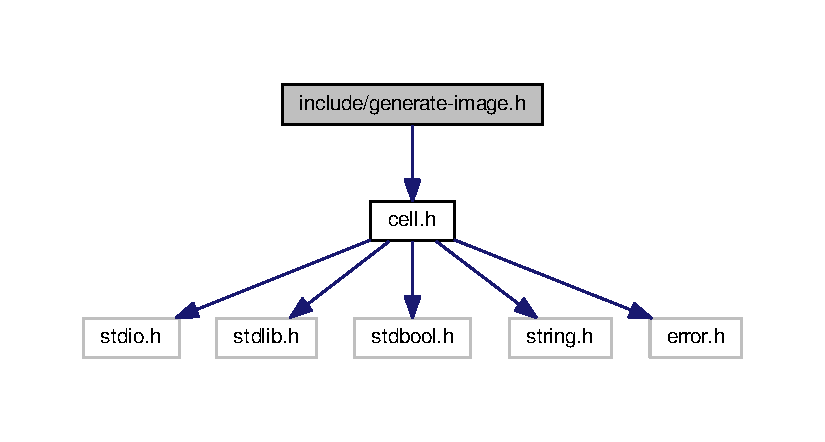
\includegraphics[width=350pt]{generate-image_8h__incl}
\end{center}
\end{figure}
This graph shows which files directly or indirectly include this file\-:\nopagebreak
\begin{figure}[H]
\begin{center}
\leavevmode
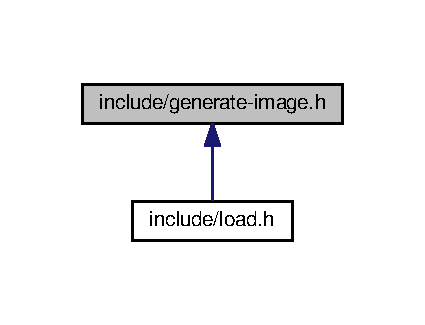
\includegraphics[width=204pt]{generate-image_8h__dep__incl}
\end{center}
\end{figure}
\subsection*{Functions}
\begin{DoxyCompactItemize}
\item 
void \hyperlink{generate-image_8h_ad873e58c1613bbcff5a45a54830b6953}{generate\-\_\-image} (\hyperlink{structproblem}{problem} $\ast$p\-\_\-prob, int number\-\_\-of\-\_\-steps, int pas)
\begin{DoxyCompactList}\small\item\em Generate the image of the problem. \end{DoxyCompactList}\item 
int \hyperlink{generate-image_8h_ac3afc5bb6983d9c71d005805520d9dfc}{number\-\_\-figures} (int number)
\begin{DoxyCompactList}\small\item\em Gives the number of figures in the number. \end{DoxyCompactList}\end{DoxyCompactItemize}


\subsection{Detailed Description}
Enable to generate an image. \begin{DoxyAuthor}{Author}
Maxence Faldor
\end{DoxyAuthor}
Composed of\-:
\begin{DoxyItemize}
\item a function to generate an image.
\item a function to get the number of figures in a number. 
\end{DoxyItemize}

\subsection{Function Documentation}
\hypertarget{generate-image_8h_ad873e58c1613bbcff5a45a54830b6953}{\index{generate-\/image.\-h@{generate-\/image.\-h}!generate\-\_\-image@{generate\-\_\-image}}
\index{generate\-\_\-image@{generate\-\_\-image}!generate-image.h@{generate-\/image.\-h}}
\subsubsection[{generate\-\_\-image}]{\setlength{\rightskip}{0pt plus 5cm}void generate\-\_\-image (
\begin{DoxyParamCaption}
\item[{{\bf problem} $\ast$}]{p\-\_\-prob, }
\item[{int}]{number\-\_\-of\-\_\-steps, }
\item[{int}]{pas}
\end{DoxyParamCaption}
)}}\label{generate-image_8h_ad873e58c1613bbcff5a45a54830b6953}


Generate the image of the problem. 


\begin{DoxyParams}{Parameters}
{\em p\-\_\-prob} & a pointer to the problem. \\
\hline
{\em number\-\_\-of\-\_\-steps} & number of steps of the problem. \\
\hline
{\em pas} & step of the problem.\\
\hline
\end{DoxyParams}
\begin{DoxyPostcond}{Postcondition}
Generate an image in the ppm format representing the problem. 
\end{DoxyPostcond}
\hypertarget{generate-image_8h_ac3afc5bb6983d9c71d005805520d9dfc}{\index{generate-\/image.\-h@{generate-\/image.\-h}!number\-\_\-figures@{number\-\_\-figures}}
\index{number\-\_\-figures@{number\-\_\-figures}!generate-image.h@{generate-\/image.\-h}}
\subsubsection[{number\-\_\-figures}]{\setlength{\rightskip}{0pt plus 5cm}int number\-\_\-figures (
\begin{DoxyParamCaption}
\item[{int}]{number}
\end{DoxyParamCaption}
)}}\label{generate-image_8h_ac3afc5bb6983d9c71d005805520d9dfc}


Gives the number of figures in the number. 


\begin{DoxyParams}{Parameters}
{\em number} & A number of int type.\\
\hline
\end{DoxyParams}
\begin{DoxyReturn}{Returns}
The number of figures in number. 
\end{DoxyReturn}

\hypertarget{load_8h}{\section{include/load.h File Reference}
\label{load_8h}\index{include/load.\-h@{include/load.\-h}}
}


Enable to load an image.  


{\ttfamily \#include \char`\"{}generate-\/image.\-h\char`\"{}}\\*
Include dependency graph for load.\-h\-:\nopagebreak
\begin{figure}[H]
\begin{center}
\leavevmode
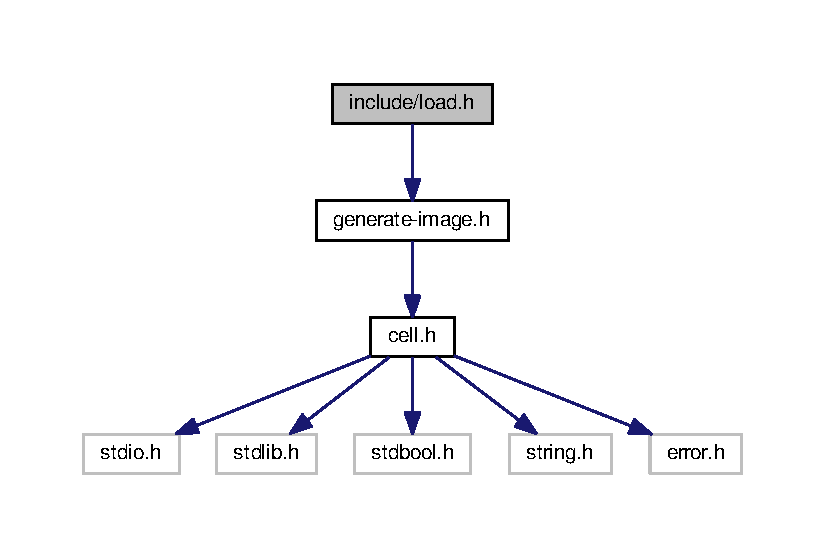
\includegraphics[width=350pt]{load_8h__incl}
\end{center}
\end{figure}
\subsection*{Functions}
\begin{DoxyCompactItemize}
\item 
\hyperlink{structproblem}{problem} $\ast$ \hyperlink{load_8h_a49966de5abd3597681b2a27a2430a11a}{load\-\_\-problem} (int argc, char $\ast$$\ast$argv)
\begin{DoxyCompactList}\small\item\em Load a problem from a .txt file. \end{DoxyCompactList}\end{DoxyCompactItemize}


\subsection{Detailed Description}
Enable to load an image. \begin{DoxyAuthor}{Author}
Maxence Faldor
\end{DoxyAuthor}
Composed of\-:
\begin{DoxyItemize}
\item a function to load a data file .txt representing the initial state of a problem. 
\end{DoxyItemize}

\subsection{Function Documentation}
\hypertarget{load_8h_a49966de5abd3597681b2a27a2430a11a}{\index{load.\-h@{load.\-h}!load\-\_\-problem@{load\-\_\-problem}}
\index{load\-\_\-problem@{load\-\_\-problem}!load.h@{load.\-h}}
\subsubsection[{load\-\_\-problem}]{\setlength{\rightskip}{0pt plus 5cm}{\bf problem}$\ast$ load\-\_\-problem (
\begin{DoxyParamCaption}
\item[{int}]{argc, }
\item[{char $\ast$$\ast$}]{argv}
\end{DoxyParamCaption}
)}}\label{load_8h_a49966de5abd3597681b2a27a2430a11a}


Load a problem from a .txt file. 


\begin{DoxyParams}{Parameters}
{\em argc} & An int given in the terminal \\
\hline
{\em argv} & A char$\ast$$\ast$ given in the terminal\\
\hline
\end{DoxyParams}
\begin{DoxyReturn}{Returns}
A pointer to a problem with a population and parameters loaded from a .txt file. 
\end{DoxyReturn}

%--- End generated contents ---

% Index
\newpage
\phantomsection
\addcontentsline{toc}{part}{Index}
\printindex

\end{document}
